\documentclass[11pt]{article}
\usepackage[english]{babel}
\usepackage[utf8]{inputenc}
\usepackage{fancyhdr}
\usepackage{graphicx}

\def\Name{Ran Liao}
\def\Topic{Capability Maturity Models}

\title{\textbf{\Topic}}
\author{\Name}
\markboth{Notes on \Topic\ }{Notes on \Topic\ }
\date{\today}
 
\pagestyle{fancy}
\fancyhf{}
\rhead{\date{\today} }
\lhead{Notes on \Topic\ }
\rfoot{\thepage}

\textheight=9in
%\textwidth=6.5in
\topmargin=-.75in
%\oddsidemargin=0in
%\evensidemargin=0in
 
\begin{document}
\maketitle
\noindent\makebox[\linewidth]{\rule[8pt]{5in}{0.5pt}}

\section*{Software Capability Maturity Models}

\begin{figure}[h]
	\centering
	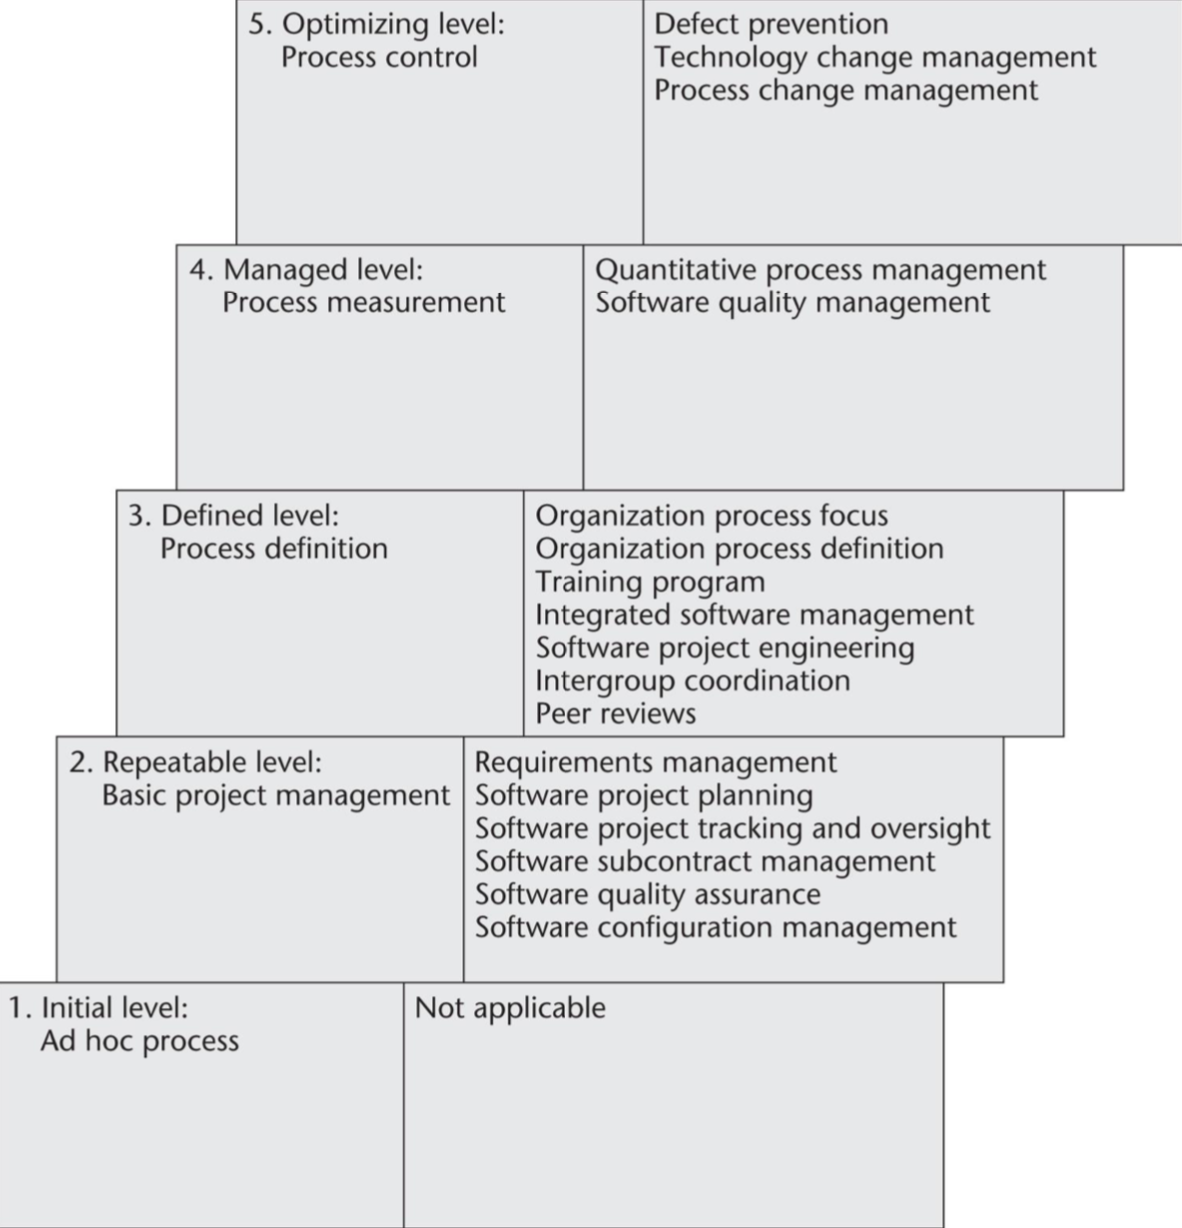
\includegraphics[width=0.9\linewidth]{images/SW-CMM.png}
	\caption{Software Capability Maturity Models}
	\label{fig:SW-CMM}
\end{figure}

\begin{enumerate}

	\item \textbf{Initial Level - Ad hoc approach}
	
	\begin{itemize}
		\item The entire process is unpredictable.
		\item Management consists of responses to crises.
	\end{itemize}

	\item \textbf{Repeatable Level - Basic software management}
	
	\begin{itemize}
		\item Management decisions should be made on the basis of previous experience with similar products.
		\item Measurements (“metrics”) are made.
		\item Problems are identified, immediate corrective action is taken.
	\end{itemize}
	
	\item \textbf{Defined Level - The software process is fully documented}
	
	\begin{itemize}
		\item The software process is fully documented. 
		\item Managerial and technical aspects are clearly defined. 
		\item Continual efforts are made to improve quality and productivity. 
		\item Reviews are performed to improve software quality. 
		\item CASE environments are applicable now.
	\end{itemize}

	\item \textbf{Managed Level - Quality and productivity goals are set}
	
	\begin{itemize}
		\item Quality and productivity are continually monitored.
		\item Statistical quality controls are in place.
	\end{itemize}

	\item \textbf{Optimizing Level}

	\begin{itemize}
		\item Statistical quality and process controls.
		\item Feedback of knowledge from each project to the next.
	\end{itemize}

\end{enumerate}





\end{document}